% SOURCE: edit-harness/results/frame_a/cells/cell_*_real_MIX_B_*.json
% !TEX encoding = UTF-8 Unicode
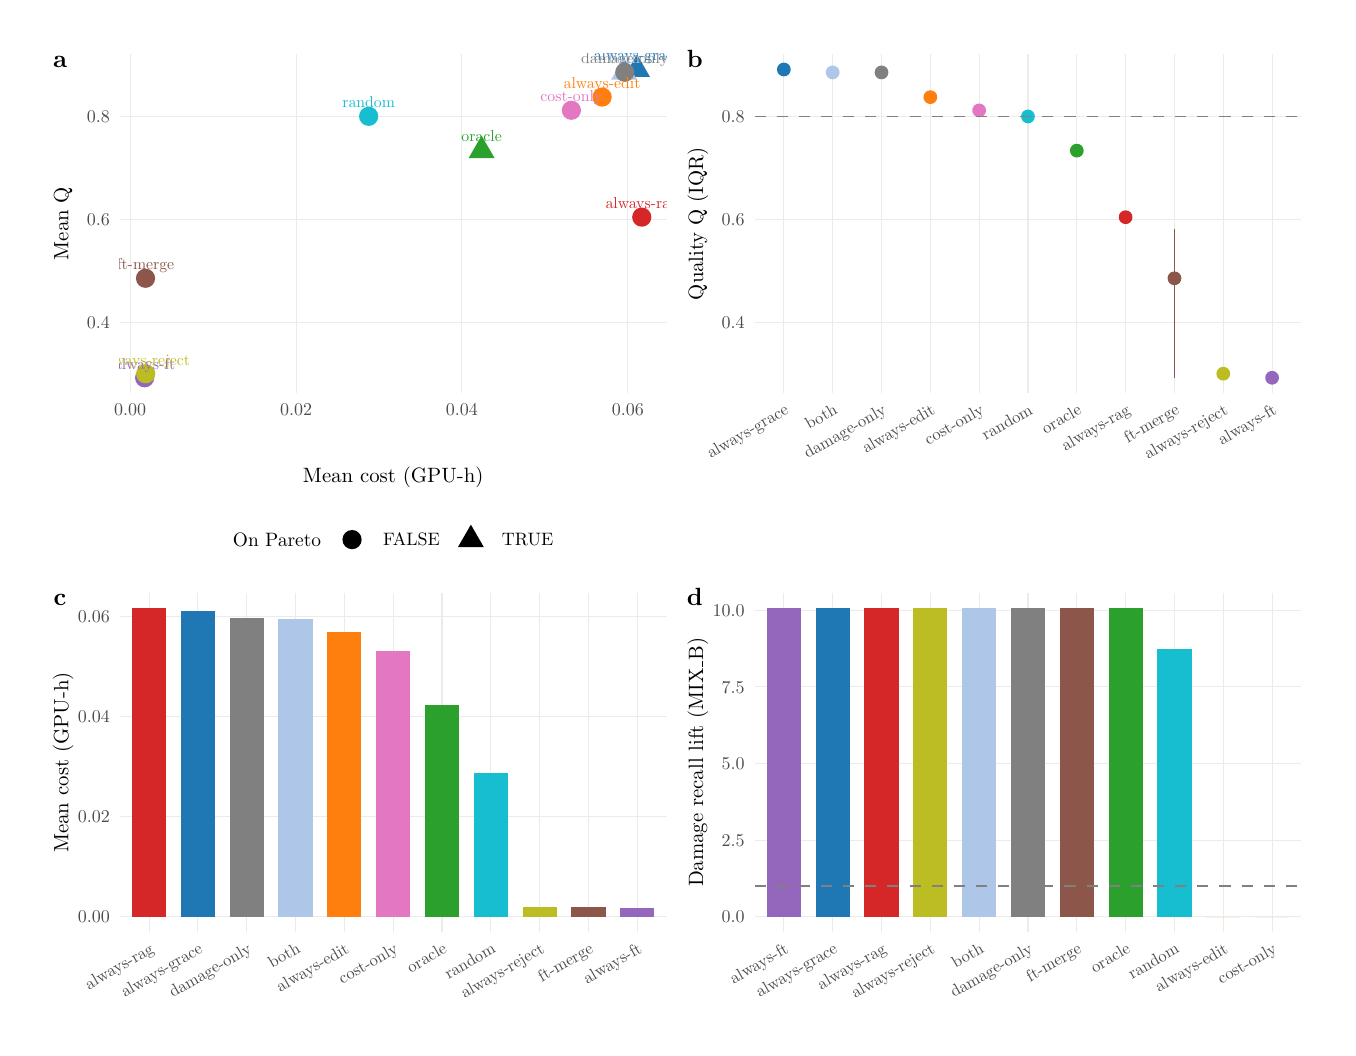
\begin{tikzpicture}[x=1pt,y=1pt]
\definecolor{fillColor}{RGB}{255,255,255}
\path[use as bounding box,fill=fillColor,fill opacity=0.00] (0,0) rectangle (469.75,361.35);
\begin{scope}
\path[clip] (  0.00,  0.00) rectangle (469.75,361.35);
\definecolor{drawColor}{RGB}{255,255,255}
\definecolor{fillColor}{RGB}{255,255,255}

\path[draw=drawColor,line width= 0.6pt,line join=round,line cap=round,fill=fillColor] (  0.00,  0.00) rectangle (469.75,361.35);
\end{scope}
\begin{scope}
\path[clip] (  5.50,161.14) rectangle (234.88,355.85);
\definecolor{fillColor}{RGB}{255,255,255}

\path[fill=fillColor] (  5.50,161.14) rectangle (234.88,355.85);
\end{scope}
\begin{scope}
\path[clip] (234.88,161.14) rectangle (464.25,355.85);
\definecolor{fillColor}{RGB}{255,255,255}

\path[fill=fillColor] (234.88,161.14) rectangle (464.25,355.85);
\end{scope}
\begin{scope}
\path[clip] (  5.50,  5.50) rectangle (234.88,161.14);
\definecolor{fillColor}{RGB}{255,255,255}

\path[fill=fillColor] (  5.50,  5.50) rectangle (234.88,161.14);
\end{scope}
\begin{scope}
\path[clip] (234.88,  5.50) rectangle (464.25,161.14);
\definecolor{fillColor}{RGB}{255,255,255}

\path[fill=fillColor] (234.88,  5.50) rectangle (464.25,161.14);
\end{scope}
\begin{scope}
\path[clip] ( 33.28,229.26) rectangle (230.88,351.85);
\definecolor{drawColor}{gray}{0.92}

\path[draw=drawColor,line width= 0.4pt,line join=round] ( 33.28,254.91) --
	(230.88,254.91);

\path[draw=drawColor,line width= 0.4pt,line join=round] ( 33.28,292.13) --
	(230.88,292.13);

\path[draw=drawColor,line width= 0.4pt,line join=round] ( 33.28,329.36) --
	(230.88,329.36);

\path[draw=drawColor,line width= 0.4pt,line join=round] ( 37.05,229.26) --
	( 37.05,351.85);

\path[draw=drawColor,line width= 0.4pt,line join=round] ( 96.98,229.26) --
	( 96.98,351.85);

\path[draw=drawColor,line width= 0.4pt,line join=round] (156.92,229.26) --
	(156.92,351.85);

\path[draw=drawColor,line width= 0.4pt,line join=round] (216.85,229.26) --
	(216.85,351.85);
\definecolor{fillColor}{RGB}{255,127,14}

\path[fill=fillColor] (207.57,336.28) circle (  3.47);
\definecolor{fillColor}{RGB}{148,103,189}

\path[fill=fillColor] ( 42.26,234.83) circle (  3.47);
\definecolor{fillColor}{RGB}{31,119,180}

\path[fill=fillColor] (220.19,351.68) --
	(224.86,343.58) --
	(215.51,343.58) --
	cycle;
\definecolor{fillColor}{RGB}{214,39,40}

\path[fill=fillColor] (221.90,292.88) circle (  3.47);
\definecolor{fillColor}{RGB}{188,189,34}

\path[fill=fillColor] ( 42.65,236.30) circle (  3.47);
\definecolor{fillColor}{RGB}{174,199,232}

\path[fill=fillColor] (215.49,350.63) --
	(220.16,342.53) --
	(210.81,342.53) --
	cycle;
\definecolor{fillColor}{RGB}{227,119,194}

\path[fill=fillColor] (196.47,331.50) circle (  3.47);
\definecolor{fillColor}{gray}{0.50}

\path[fill=fillColor] (215.75,345.23) circle (  3.47);
\definecolor{fillColor}{RGB}{140,86,75}

\path[fill=fillColor] ( 42.58,270.79) circle (  3.47);
\definecolor{fillColor}{RGB}{44,160,44}

\path[fill=fillColor] (164.02,322.35) --
	(168.70,314.25) --
	(159.35,314.25) --
	cycle;
\definecolor{fillColor}{RGB}{23,190,207}

\path[fill=fillColor] (123.21,329.31) circle (  3.47);
\definecolor{drawColor}{RGB}{255,127,14}

\node[text=drawColor,anchor=base,inner sep=0pt, outer sep=0pt, scale=  0.57] at (207.57,339.42) {always-edit};
\definecolor{drawColor}{RGB}{148,103,189}

\node[text=drawColor,anchor=base,inner sep=0pt, outer sep=0pt, scale=  0.57] at ( 42.26,237.96) {always-ft};
\definecolor{drawColor}{RGB}{31,119,180}

\node[text=drawColor,anchor=base,inner sep=0pt, outer sep=0pt, scale=  0.57] at (220.19,349.41) {always-grace};
\definecolor{drawColor}{RGB}{214,39,40}

\node[text=drawColor,anchor=base,inner sep=0pt, outer sep=0pt, scale=  0.57] at (221.90,296.01) {always-rag};
\definecolor{drawColor}{RGB}{188,189,34}

\node[text=drawColor,anchor=base,inner sep=0pt, outer sep=0pt, scale=  0.57] at ( 42.65,239.43) {always-reject};
\definecolor{drawColor}{RGB}{174,199,232}

\node[text=drawColor,anchor=base,inner sep=0pt, outer sep=0pt, scale=  0.57] at (215.49,348.37) {both};
\definecolor{drawColor}{RGB}{227,119,194}

\node[text=drawColor,anchor=base,inner sep=0pt, outer sep=0pt, scale=  0.57] at (196.47,334.64) {cost-only};
\definecolor{drawColor}{gray}{0.50}

\node[text=drawColor,anchor=base,inner sep=0pt, outer sep=0pt, scale=  0.57] at (215.75,348.37) {damage-only};
\definecolor{drawColor}{RGB}{140,86,75}

\node[text=drawColor,anchor=base,inner sep=0pt, outer sep=0pt, scale=  0.57] at ( 42.58,273.93) {ft-merge};
\definecolor{drawColor}{RGB}{44,160,44}

\node[text=drawColor,anchor=base,inner sep=0pt, outer sep=0pt, scale=  0.57] at (164.02,320.08) {oracle};
\definecolor{drawColor}{RGB}{23,190,207}

\node[text=drawColor,anchor=base,inner sep=0pt, outer sep=0pt, scale=  0.57] at (123.21,332.45) {random};
\end{scope}
\begin{scope}
\path[clip] (  0.00,  0.00) rectangle (469.75,361.35);
\definecolor{drawColor}{gray}{0.30}

\node[text=drawColor,anchor=base east,inner sep=0pt, outer sep=0pt, scale=  0.65] at ( 29.68,252.67) {0.4};

\node[text=drawColor,anchor=base east,inner sep=0pt, outer sep=0pt, scale=  0.65] at ( 29.68,289.89) {0.6};

\node[text=drawColor,anchor=base east,inner sep=0pt, outer sep=0pt, scale=  0.65] at ( 29.68,327.12) {0.8};
\end{scope}
\begin{scope}
\path[clip] (  0.00,  0.00) rectangle (469.75,361.35);
\definecolor{drawColor}{gray}{0.30}

\node[text=drawColor,anchor=base,inner sep=0pt, outer sep=0pt, scale=  0.65] at ( 37.05,221.18) {0.00};

\node[text=drawColor,anchor=base,inner sep=0pt, outer sep=0pt, scale=  0.65] at ( 96.98,221.18) {0.02};

\node[text=drawColor,anchor=base,inner sep=0pt, outer sep=0pt, scale=  0.65] at (156.92,221.18) {0.04};

\node[text=drawColor,anchor=base,inner sep=0pt, outer sep=0pt, scale=  0.65] at (216.85,221.18) {0.06};
\end{scope}
\begin{scope}
\path[clip] (  0.00,  0.00) rectangle (469.75,361.35);
\definecolor{drawColor}{RGB}{0,0,0}

\node[text=drawColor,anchor=base,inner sep=0pt, outer sep=0pt, scale=  0.75] at (132.08,197.05) {Mean cost (GPU-h)};
\end{scope}
\begin{scope}
\path[clip] (  0.00,  0.00) rectangle (469.75,361.35);
\definecolor{drawColor}{RGB}{0,0,0}

\node[text=drawColor,rotate= 90.00,anchor=base,inner sep=0pt, outer sep=0pt, scale=  0.75] at ( 14.67,290.55) {Mean Q};
\end{scope}
\begin{scope}
\path[clip] (  0.00,  0.00) rectangle (469.75,361.35);
\definecolor{drawColor}{RGB}{0,0,0}

\node[text=drawColor,anchor=base west,inner sep=0pt, outer sep=0pt, scale=  0.70] at ( 74.18,173.95) {On Pareto};
\end{scope}
\begin{scope}
\path[clip] (  0.00,  0.00) rectangle (469.75,361.35);
\definecolor{fillColor}{RGB}{0,0,0}

\path[fill=fillColor] (117.21,176.36) circle (  3.47);
\end{scope}
\begin{scope}
\path[clip] (  0.00,  0.00) rectangle (469.75,361.35);
\definecolor{fillColor}{RGB}{0,0,0}

\path[fill=fillColor] (160.15,181.76) --
	(164.83,173.66) --
	(155.48,173.66) --
	cycle;
\end{scope}
\begin{scope}
\path[clip] (  0.00,  0.00) rectangle (469.75,361.35);
\definecolor{drawColor}{RGB}{0,0,0}

\node[text=drawColor,anchor=base west,inner sep=0pt, outer sep=0pt, scale=  0.65] at (128.44,174.12) {FALSE};
\end{scope}
\begin{scope}
\path[clip] (  0.00,  0.00) rectangle (469.75,361.35);
\definecolor{drawColor}{RGB}{0,0,0}

\node[text=drawColor,anchor=base west,inner sep=0pt, outer sep=0pt, scale=  0.65] at (171.38,174.12) {TRUE};
\end{scope}
\begin{scope}
\path[clip] (  0.00,  0.00) rectangle (469.75,361.35);
\definecolor{drawColor}{RGB}{0,0,0}

\node[text=drawColor,anchor=base,inner sep=0pt, outer sep=0pt, scale=  0.90] at ( 11.71,346.88) {\bfseries a};
\end{scope}
\begin{scope}
\path[clip] (262.65,229.26) rectangle (460.25,351.85);
\definecolor{drawColor}{gray}{0.92}

\path[draw=drawColor,line width= 0.4pt,line join=round] (262.65,254.91) --
	(460.25,254.91);

\path[draw=drawColor,line width= 0.4pt,line join=round] (262.65,292.11) --
	(460.25,292.11);

\path[draw=drawColor,line width= 0.4pt,line join=round] (262.65,329.32) --
	(460.25,329.32);

\path[draw=drawColor,line width= 0.4pt,line join=round] (273.24,229.26) --
	(273.24,351.85);

\path[draw=drawColor,line width= 0.4pt,line join=round] (290.88,229.26) --
	(290.88,351.85);

\path[draw=drawColor,line width= 0.4pt,line join=round] (308.53,229.26) --
	(308.53,351.85);

\path[draw=drawColor,line width= 0.4pt,line join=round] (326.17,229.26) --
	(326.17,351.85);

\path[draw=drawColor,line width= 0.4pt,line join=round] (343.81,229.26) --
	(343.81,351.85);

\path[draw=drawColor,line width= 0.4pt,line join=round] (361.45,229.26) --
	(361.45,351.85);

\path[draw=drawColor,line width= 0.4pt,line join=round] (379.10,229.26) --
	(379.10,351.85);

\path[draw=drawColor,line width= 0.4pt,line join=round] (396.74,229.26) --
	(396.74,351.85);

\path[draw=drawColor,line width= 0.4pt,line join=round] (414.38,229.26) --
	(414.38,351.85);

\path[draw=drawColor,line width= 0.4pt,line join=round] (432.03,229.26) --
	(432.03,351.85);

\path[draw=drawColor,line width= 0.4pt,line join=round] (449.67,229.26) --
	(449.67,351.85);
\definecolor{drawColor}{RGB}{255,127,14}

\path[draw=drawColor,line width= 0.4pt,line join=round] (326.17,335.69) -- (326.17,336.59);
\definecolor{drawColor}{RGB}{148,103,189}

\path[draw=drawColor,line width= 0.4pt,line join=round] (449.67,234.83) -- (449.67,234.85);
\definecolor{drawColor}{RGB}{31,119,180}

\path[draw=drawColor,line width= 0.4pt,line join=round] (273.24,346.13) -- (273.24,346.28);
\definecolor{drawColor}{RGB}{214,39,40}

\path[draw=drawColor,line width= 0.4pt,line join=round] (396.74,292.78) -- (396.74,293.00);
\definecolor{drawColor}{RGB}{188,189,34}

\path[draw=drawColor,line width= 0.4pt,line join=round] (432.03,236.31) -- (432.03,236.31);
\definecolor{drawColor}{RGB}{174,199,232}

\path[draw=drawColor,line width= 0.4pt,line join=round] (290.88,345.08) -- (290.88,345.26);
\definecolor{drawColor}{RGB}{227,119,194}

\path[draw=drawColor,line width= 0.4pt,line join=round] (343.81,331.01) -- (343.81,332.10);
\definecolor{drawColor}{gray}{0.50}

\path[draw=drawColor,line width= 0.4pt,line join=round] (308.53,345.08) -- (308.53,345.26);
\definecolor{drawColor}{RGB}{140,86,75}

\path[draw=drawColor,line width= 0.4pt,line join=round] (414.38,234.85) -- (414.38,288.75);
\definecolor{drawColor}{RGB}{44,160,44}

\path[draw=drawColor,line width= 0.4pt,line join=round] (379.10,316.81) -- (379.10,317.04);
\definecolor{drawColor}{RGB}{23,190,207}

\path[draw=drawColor,line width= 0.4pt,line join=round] (361.45,328.54) -- (361.45,330.01);
\definecolor{drawColor}{RGB}{255,127,14}
\definecolor{fillColor}{RGB}{255,127,14}

\path[draw=drawColor,line width= 0.5pt,line join=round,line cap=round,fill=fillColor] (326.17,336.24) circle (  2.23);
\definecolor{drawColor}{RGB}{148,103,189}
\definecolor{fillColor}{RGB}{148,103,189}

\path[draw=drawColor,line width= 0.5pt,line join=round,line cap=round,fill=fillColor] (449.67,234.84) circle (  2.23);
\definecolor{drawColor}{RGB}{31,119,180}
\definecolor{fillColor}{RGB}{31,119,180}

\path[draw=drawColor,line width= 0.5pt,line join=round,line cap=round,fill=fillColor] (273.24,346.23) circle (  2.23);
\definecolor{drawColor}{RGB}{214,39,40}
\definecolor{fillColor}{RGB}{214,39,40}

\path[draw=drawColor,line width= 0.5pt,line join=round,line cap=round,fill=fillColor] (396.74,292.86) circle (  2.23);
\definecolor{drawColor}{RGB}{188,189,34}
\definecolor{fillColor}{RGB}{188,189,34}

\path[draw=drawColor,line width= 0.5pt,line join=round,line cap=round,fill=fillColor] (432.03,236.31) circle (  2.23);
\definecolor{drawColor}{RGB}{174,199,232}
\definecolor{fillColor}{RGB}{174,199,232}

\path[draw=drawColor,line width= 0.5pt,line join=round,line cap=round,fill=fillColor] (290.88,345.18) circle (  2.23);
\definecolor{drawColor}{RGB}{227,119,194}
\definecolor{fillColor}{RGB}{227,119,194}

\path[draw=drawColor,line width= 0.5pt,line join=round,line cap=round,fill=fillColor] (343.81,331.46) circle (  2.23);
\definecolor{drawColor}{gray}{0.50}
\definecolor{fillColor}{gray}{0.50}

\path[draw=drawColor,line width= 0.5pt,line join=round,line cap=round,fill=fillColor] (308.53,345.18) circle (  2.23);
\definecolor{drawColor}{RGB}{140,86,75}
\definecolor{fillColor}{RGB}{140,86,75}

\path[draw=drawColor,line width= 0.5pt,line join=round,line cap=round,fill=fillColor] (414.38,270.78) circle (  2.23);
\definecolor{drawColor}{RGB}{44,160,44}
\definecolor{fillColor}{RGB}{44,160,44}

\path[draw=drawColor,line width= 0.5pt,line join=round,line cap=round,fill=fillColor] (379.10,316.91) circle (  2.23);
\definecolor{drawColor}{RGB}{23,190,207}
\definecolor{fillColor}{RGB}{23,190,207}

\path[draw=drawColor,line width= 0.5pt,line join=round,line cap=round,fill=fillColor] (361.45,329.27) circle (  2.23);
\definecolor{drawColor}{gray}{0.50}

\path[draw=drawColor,line width= 0.5pt,dash pattern=on 4pt off 4pt ,line join=round] (262.65,329.27) -- (460.25,329.27);
\end{scope}
\begin{scope}
\path[clip] (  0.00,  0.00) rectangle (469.75,361.35);
\definecolor{drawColor}{gray}{0.30}

\node[text=drawColor,anchor=base east,inner sep=0pt, outer sep=0pt, scale=  0.65] at (259.05,252.67) {0.4};

\node[text=drawColor,anchor=base east,inner sep=0pt, outer sep=0pt, scale=  0.65] at (259.05,289.87) {0.6};

\node[text=drawColor,anchor=base east,inner sep=0pt, outer sep=0pt, scale=  0.65] at (259.05,327.08) {0.8};
\end{scope}
\begin{scope}
\path[clip] (  0.00,  0.00) rectangle (469.75,361.35);
\definecolor{drawColor}{gray}{0.30}

\node[text=drawColor,rotate= 30.00,anchor=base east,inner sep=0pt, outer sep=0pt, scale=  0.60] at (275.31,222.08) {always-grace};

\node[text=drawColor,rotate= 30.00,anchor=base east,inner sep=0pt, outer sep=0pt, scale=  0.60] at (292.95,222.08) {both};

\node[text=drawColor,rotate= 30.00,anchor=base east,inner sep=0pt, outer sep=0pt, scale=  0.60] at (310.59,222.08) {damage-only};

\node[text=drawColor,rotate= 30.00,anchor=base east,inner sep=0pt, outer sep=0pt, scale=  0.60] at (328.23,222.08) {always-edit};

\node[text=drawColor,rotate= 30.00,anchor=base east,inner sep=0pt, outer sep=0pt, scale=  0.60] at (345.88,222.08) {cost-only};

\node[text=drawColor,rotate= 30.00,anchor=base east,inner sep=0pt, outer sep=0pt, scale=  0.60] at (363.52,222.08) {random};

\node[text=drawColor,rotate= 30.00,anchor=base east,inner sep=0pt, outer sep=0pt, scale=  0.60] at (381.16,222.08) {oracle};

\node[text=drawColor,rotate= 30.00,anchor=base east,inner sep=0pt, outer sep=0pt, scale=  0.60] at (398.81,222.08) {always-rag};

\node[text=drawColor,rotate= 30.00,anchor=base east,inner sep=0pt, outer sep=0pt, scale=  0.60] at (416.45,222.08) {ft-merge};

\node[text=drawColor,rotate= 30.00,anchor=base east,inner sep=0pt, outer sep=0pt, scale=  0.60] at (434.09,222.08) {always-reject};

\node[text=drawColor,rotate= 30.00,anchor=base east,inner sep=0pt, outer sep=0pt, scale=  0.60] at (451.74,222.08) {always-ft};
\end{scope}
\begin{scope}
\path[clip] (  0.00,  0.00) rectangle (469.75,361.35);
\definecolor{drawColor}{RGB}{0,0,0}

\node[text=drawColor,rotate= 90.00,anchor=base,inner sep=0pt, outer sep=0pt, scale=  0.75] at (244.04,290.55) {Quality Q (IQR)};
\end{scope}
\begin{scope}
\path[clip] (  0.00,  0.00) rectangle (469.75,361.35);
\definecolor{drawColor}{RGB}{0,0,0}

\node[text=drawColor,anchor=base,inner sep=0pt, outer sep=0pt, scale=  0.90] at (241.09,346.88) {\bfseries b};
\end{scope}
\begin{scope}
\path[clip] ( 33.28, 34.54) rectangle (230.88,157.14);
\definecolor{drawColor}{gray}{0.92}

\path[draw=drawColor,line width= 0.4pt,line join=round] ( 33.28, 40.12) --
	(230.88, 40.12);

\path[draw=drawColor,line width= 0.4pt,line join=round] ( 33.28, 76.25) --
	(230.88, 76.25);

\path[draw=drawColor,line width= 0.4pt,line join=round] ( 33.28,112.39) --
	(230.88,112.39);

\path[draw=drawColor,line width= 0.4pt,line join=round] ( 33.28,148.52) --
	(230.88,148.52);

\path[draw=drawColor,line width= 0.4pt,line join=round] ( 43.86, 34.54) --
	( 43.86,157.14);

\path[draw=drawColor,line width= 0.4pt,line join=round] ( 61.50, 34.54) --
	( 61.50,157.14);

\path[draw=drawColor,line width= 0.4pt,line join=round] ( 79.15, 34.54) --
	( 79.15,157.14);

\path[draw=drawColor,line width= 0.4pt,line join=round] ( 96.79, 34.54) --
	( 96.79,157.14);

\path[draw=drawColor,line width= 0.4pt,line join=round] (114.43, 34.54) --
	(114.43,157.14);

\path[draw=drawColor,line width= 0.4pt,line join=round] (132.08, 34.54) --
	(132.08,157.14);

\path[draw=drawColor,line width= 0.4pt,line join=round] (149.72, 34.54) --
	(149.72,157.14);

\path[draw=drawColor,line width= 0.4pt,line join=round] (167.36, 34.54) --
	(167.36,157.14);

\path[draw=drawColor,line width= 0.4pt,line join=round] (185.01, 34.54) --
	(185.01,157.14);

\path[draw=drawColor,line width= 0.4pt,line join=round] (202.65, 34.54) --
	(202.65,157.14);

\path[draw=drawColor,line width= 0.4pt,line join=round] (220.29, 34.54) --
	(220.29,157.14);
\definecolor{fillColor}{RGB}{255,127,14}

\path[fill=fillColor] (108.26, 40.12) rectangle (120.61,142.93);
\definecolor{fillColor}{RGB}{148,103,189}

\path[fill=fillColor] (214.12, 40.12) rectangle (226.47, 43.26);
\definecolor{fillColor}{RGB}{31,119,180}

\path[fill=fillColor] ( 55.33, 40.12) rectangle ( 67.68,150.53);
\definecolor{fillColor}{RGB}{214,39,40}

\path[fill=fillColor] ( 37.69, 40.12) rectangle ( 50.04,151.56);
\definecolor{fillColor}{RGB}{188,189,34}

\path[fill=fillColor] (178.83, 40.12) rectangle (191.18, 43.49);
\definecolor{fillColor}{RGB}{174,199,232}

\path[fill=fillColor] ( 90.62, 40.12) rectangle (102.97,147.70);
\definecolor{fillColor}{RGB}{227,119,194}

\path[fill=fillColor] (125.90, 40.12) rectangle (138.25,136.23);
\definecolor{fillColor}{gray}{0.50}

\path[fill=fillColor] ( 72.97, 40.12) rectangle ( 85.32,147.86);
\definecolor{fillColor}{RGB}{140,86,75}

\path[fill=fillColor] (196.47, 40.12) rectangle (208.82, 43.45);
\definecolor{fillColor}{RGB}{44,160,44}

\path[fill=fillColor] (143.54, 40.12) rectangle (155.89,116.67);
\definecolor{fillColor}{RGB}{23,190,207}

\path[fill=fillColor] (161.19, 40.12) rectangle (173.54, 92.06);
\end{scope}
\begin{scope}
\path[clip] (  0.00,  0.00) rectangle (469.75,361.35);
\definecolor{drawColor}{gray}{0.30}

\node[text=drawColor,anchor=base east,inner sep=0pt, outer sep=0pt, scale=  0.65] at ( 29.68, 37.88) {0.00};

\node[text=drawColor,anchor=base east,inner sep=0pt, outer sep=0pt, scale=  0.65] at ( 29.68, 74.01) {0.02};

\node[text=drawColor,anchor=base east,inner sep=0pt, outer sep=0pt, scale=  0.65] at ( 29.68,110.15) {0.04};

\node[text=drawColor,anchor=base east,inner sep=0pt, outer sep=0pt, scale=  0.65] at ( 29.68,146.28) {0.06};
\end{scope}
\begin{scope}
\path[clip] (  0.00,  0.00) rectangle (469.75,361.35);
\definecolor{drawColor}{gray}{0.30}

\node[text=drawColor,rotate= 30.00,anchor=base east,inner sep=0pt, outer sep=0pt, scale=  0.60] at ( 45.93, 27.36) {always-rag};

\node[text=drawColor,rotate= 30.00,anchor=base east,inner sep=0pt, outer sep=0pt, scale=  0.60] at ( 63.57, 27.36) {always-grace};

\node[text=drawColor,rotate= 30.00,anchor=base east,inner sep=0pt, outer sep=0pt, scale=  0.60] at ( 81.21, 27.36) {damage-only};

\node[text=drawColor,rotate= 30.00,anchor=base east,inner sep=0pt, outer sep=0pt, scale=  0.60] at ( 98.86, 27.36) {both};

\node[text=drawColor,rotate= 30.00,anchor=base east,inner sep=0pt, outer sep=0pt, scale=  0.60] at (116.50, 27.36) {always-edit};

\node[text=drawColor,rotate= 30.00,anchor=base east,inner sep=0pt, outer sep=0pt, scale=  0.60] at (134.14, 27.36) {cost-only};

\node[text=drawColor,rotate= 30.00,anchor=base east,inner sep=0pt, outer sep=0pt, scale=  0.60] at (151.79, 27.36) {oracle};

\node[text=drawColor,rotate= 30.00,anchor=base east,inner sep=0pt, outer sep=0pt, scale=  0.60] at (169.43, 27.36) {random};

\node[text=drawColor,rotate= 30.00,anchor=base east,inner sep=0pt, outer sep=0pt, scale=  0.60] at (187.07, 27.36) {always-reject};

\node[text=drawColor,rotate= 30.00,anchor=base east,inner sep=0pt, outer sep=0pt, scale=  0.60] at (204.71, 27.36) {ft-merge};

\node[text=drawColor,rotate= 30.00,anchor=base east,inner sep=0pt, outer sep=0pt, scale=  0.60] at (222.36, 27.36) {always-ft};
\end{scope}
\begin{scope}
\path[clip] (  0.00,  0.00) rectangle (469.75,361.35);
\definecolor{drawColor}{RGB}{0,0,0}

\node[text=drawColor,rotate= 90.00,anchor=base,inner sep=0pt, outer sep=0pt, scale=  0.75] at ( 14.67, 95.84) {Mean cost (GPU-h)};
\end{scope}
\begin{scope}
\path[clip] (  0.00,  0.00) rectangle (469.75,361.35);
\definecolor{drawColor}{RGB}{0,0,0}

\node[text=drawColor,anchor=base,inner sep=0pt, outer sep=0pt, scale=  0.90] at ( 11.71,152.55) {\bfseries c};
\end{scope}
\begin{scope}
\path[clip] (262.65, 34.54) rectangle (460.25,157.14);
\definecolor{drawColor}{gray}{0.92}

\path[draw=drawColor,line width= 0.4pt,line join=round] (262.65, 40.12) --
	(460.25, 40.12);

\path[draw=drawColor,line width= 0.4pt,line join=round] (262.65, 67.78) --
	(460.25, 67.78);

\path[draw=drawColor,line width= 0.4pt,line join=round] (262.65, 95.45) --
	(460.25, 95.45);

\path[draw=drawColor,line width= 0.4pt,line join=round] (262.65,123.12) --
	(460.25,123.12);

\path[draw=drawColor,line width= 0.4pt,line join=round] (262.65,150.78) --
	(460.25,150.78);

\path[draw=drawColor,line width= 0.4pt,line join=round] (273.24, 34.54) --
	(273.24,157.14);

\path[draw=drawColor,line width= 0.4pt,line join=round] (290.88, 34.54) --
	(290.88,157.14);

\path[draw=drawColor,line width= 0.4pt,line join=round] (308.53, 34.54) --
	(308.53,157.14);

\path[draw=drawColor,line width= 0.4pt,line join=round] (326.17, 34.54) --
	(326.17,157.14);

\path[draw=drawColor,line width= 0.4pt,line join=round] (343.81, 34.54) --
	(343.81,157.14);

\path[draw=drawColor,line width= 0.4pt,line join=round] (361.45, 34.54) --
	(361.45,157.14);

\path[draw=drawColor,line width= 0.4pt,line join=round] (379.10, 34.54) --
	(379.10,157.14);

\path[draw=drawColor,line width= 0.4pt,line join=round] (396.74, 34.54) --
	(396.74,157.14);

\path[draw=drawColor,line width= 0.4pt,line join=round] (414.38, 34.54) --
	(414.38,157.14);

\path[draw=drawColor,line width= 0.4pt,line join=round] (432.03, 34.54) --
	(432.03,157.14);

\path[draw=drawColor,line width= 0.4pt,line join=round] (449.67, 34.54) --
	(449.67,157.14);
\definecolor{fillColor}{RGB}{255,127,14}

\path[fill=fillColor] (425.85, 40.12) rectangle (438.20, 40.12);
\definecolor{fillColor}{RGB}{148,103,189}

\path[fill=fillColor] (267.06, 40.12) rectangle (279.41,151.56);
\definecolor{fillColor}{RGB}{31,119,180}

\path[fill=fillColor] (284.71, 40.12) rectangle (297.06,151.56);
\definecolor{fillColor}{RGB}{214,39,40}

\path[fill=fillColor] (302.35, 40.12) rectangle (314.70,151.56);
\definecolor{fillColor}{RGB}{188,189,34}

\path[fill=fillColor] (319.99, 40.12) rectangle (332.34,151.56);
\definecolor{fillColor}{RGB}{174,199,232}

\path[fill=fillColor] (337.64, 40.12) rectangle (349.99,151.56);
\definecolor{fillColor}{RGB}{227,119,194}

\path[fill=fillColor] (443.49, 40.12) rectangle (455.84, 40.12);
\definecolor{fillColor}{gray}{0.50}

\path[fill=fillColor] (355.28, 40.12) rectangle (367.63,151.56);
\definecolor{fillColor}{RGB}{140,86,75}

\path[fill=fillColor] (372.92, 40.12) rectangle (385.27,151.56);
\definecolor{fillColor}{RGB}{44,160,44}

\path[fill=fillColor] (390.57, 40.12) rectangle (402.92,151.56);
\definecolor{fillColor}{RGB}{23,190,207}

\path[fill=fillColor] (408.21, 40.12) rectangle (420.56,136.70);
\definecolor{drawColor}{gray}{0.50}

\path[draw=drawColor,line width= 0.5pt,dash pattern=on 4pt off 4pt ,line join=round] (262.65, 51.18) -- (460.25, 51.18);
\end{scope}
\begin{scope}
\path[clip] (  0.00,  0.00) rectangle (469.75,361.35);
\definecolor{drawColor}{gray}{0.30}

\node[text=drawColor,anchor=base east,inner sep=0pt, outer sep=0pt, scale=  0.65] at (259.05, 37.88) {0.0};

\node[text=drawColor,anchor=base east,inner sep=0pt, outer sep=0pt, scale=  0.65] at (259.05, 65.54) {2.5};

\node[text=drawColor,anchor=base east,inner sep=0pt, outer sep=0pt, scale=  0.65] at (259.05, 93.21) {5.0};

\node[text=drawColor,anchor=base east,inner sep=0pt, outer sep=0pt, scale=  0.65] at (259.05,120.88) {7.5};

\node[text=drawColor,anchor=base east,inner sep=0pt, outer sep=0pt, scale=  0.65] at (259.05,148.55) {10.0};
\end{scope}
\begin{scope}
\path[clip] (  0.00,  0.00) rectangle (469.75,361.35);
\definecolor{drawColor}{gray}{0.30}

\node[text=drawColor,rotate= 30.00,anchor=base east,inner sep=0pt, outer sep=0pt, scale=  0.60] at (275.31, 27.36) {always-ft};

\node[text=drawColor,rotate= 30.00,anchor=base east,inner sep=0pt, outer sep=0pt, scale=  0.60] at (292.95, 27.36) {always-grace};

\node[text=drawColor,rotate= 30.00,anchor=base east,inner sep=0pt, outer sep=0pt, scale=  0.60] at (310.59, 27.36) {always-rag};

\node[text=drawColor,rotate= 30.00,anchor=base east,inner sep=0pt, outer sep=0pt, scale=  0.60] at (328.23, 27.36) {always-reject};

\node[text=drawColor,rotate= 30.00,anchor=base east,inner sep=0pt, outer sep=0pt, scale=  0.60] at (345.88, 27.36) {both};

\node[text=drawColor,rotate= 30.00,anchor=base east,inner sep=0pt, outer sep=0pt, scale=  0.60] at (363.52, 27.36) {damage-only};

\node[text=drawColor,rotate= 30.00,anchor=base east,inner sep=0pt, outer sep=0pt, scale=  0.60] at (381.16, 27.36) {ft-merge};

\node[text=drawColor,rotate= 30.00,anchor=base east,inner sep=0pt, outer sep=0pt, scale=  0.60] at (398.81, 27.36) {oracle};

\node[text=drawColor,rotate= 30.00,anchor=base east,inner sep=0pt, outer sep=0pt, scale=  0.60] at (416.45, 27.36) {random};

\node[text=drawColor,rotate= 30.00,anchor=base east,inner sep=0pt, outer sep=0pt, scale=  0.60] at (434.09, 27.36) {always-edit};

\node[text=drawColor,rotate= 30.00,anchor=base east,inner sep=0pt, outer sep=0pt, scale=  0.60] at (451.74, 27.36) {cost-only};
\end{scope}
\begin{scope}
\path[clip] (  0.00,  0.00) rectangle (469.75,361.35);
\definecolor{drawColor}{RGB}{0,0,0}

\node[text=drawColor,rotate= 90.00,anchor=base,inner sep=0pt, outer sep=0pt, scale=  0.75] at (244.04, 95.84) {Damage recall lift (MIX\_B)};
\end{scope}
\begin{scope}
\path[clip] (  0.00,  0.00) rectangle (469.75,361.35);
\definecolor{drawColor}{RGB}{0,0,0}

\node[text=drawColor,anchor=base,inner sep=0pt, outer sep=0pt, scale=  0.90] at (241.09,152.55) {\bfseries d};
\end{scope}
\end{tikzpicture}
